\newpage
\chapter{Appendix}
\label{sec:Appendix}

\section*{Video-Super-Resolution using Direct Approach}
As first approach for applying \ac{TAD} to the \ac{VSR} problem it was tried to brute-force a downscaling operation directly improving the performance of an external \ac{VSR} model. Therefore, as shown in \myfigref{fig:architecture_video_direct}, the training loss is defined based on the upscaling performance of the external model, which was fixed during the training procedure. However, since other approaches could successfully solve the \ac{VSR} task this approach was discarded.

\begin{figure}[!ht]
	\centering
	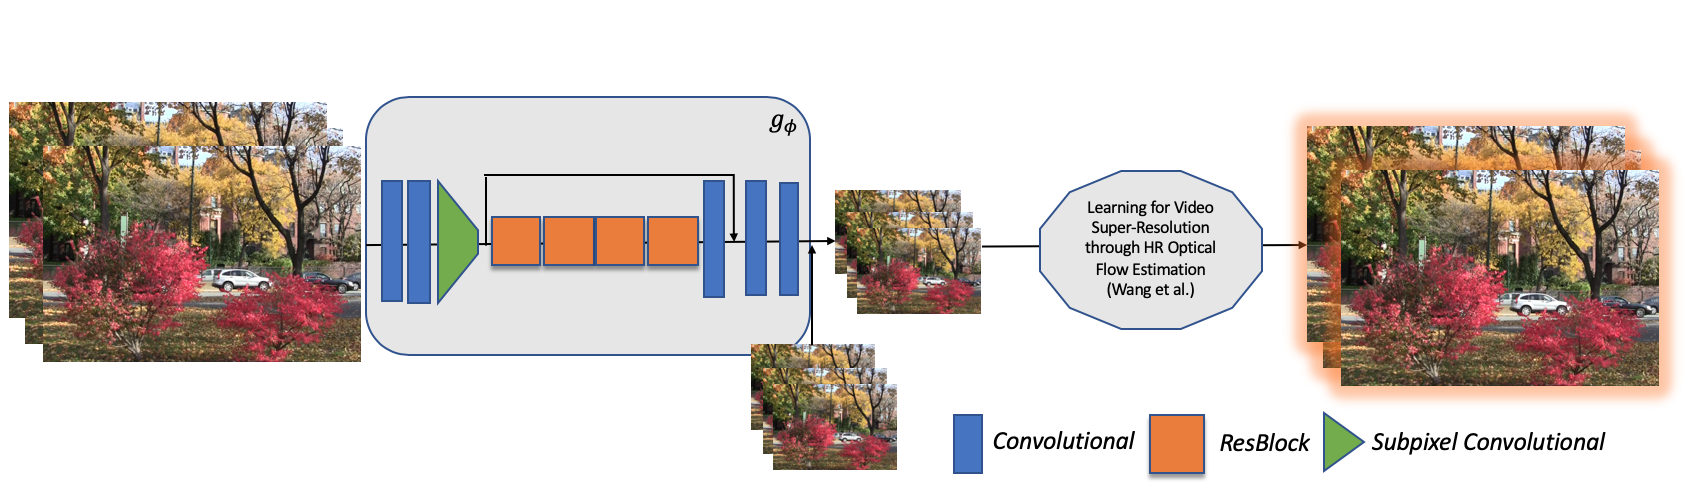
\includegraphics[width=14cm]{figures/architecture_video_direct.png}
	\caption{Design for \ac{TAD} video super-resolution architecture for direct improvement of downscaling operation. }
  \label{fig:architecture_video_direct}
\end{figure}

\section*{Video-Super-Resolution using Optical Flow Reconstruction}
Another approach that was tried in order to apply \ac{TAD} on \ac{VSR} was to find a low-dimensional representation that is optimal to reconstruct the optical flow. \myfigref{fig:architecture_video_flow} indicates the design for this approach, which was trained using the UCL optical flow dataset (\cite{ADAEMFOF}) and the OpenCV Farneback dense optical flow function (since easily available for a conceptual test). Unfortunately, the approach did not converge to useful representation. Since other approaches could successfully solve the \ac{VSR} task this approach was discarded.

\begin{figure}[!ht]
	\centering
	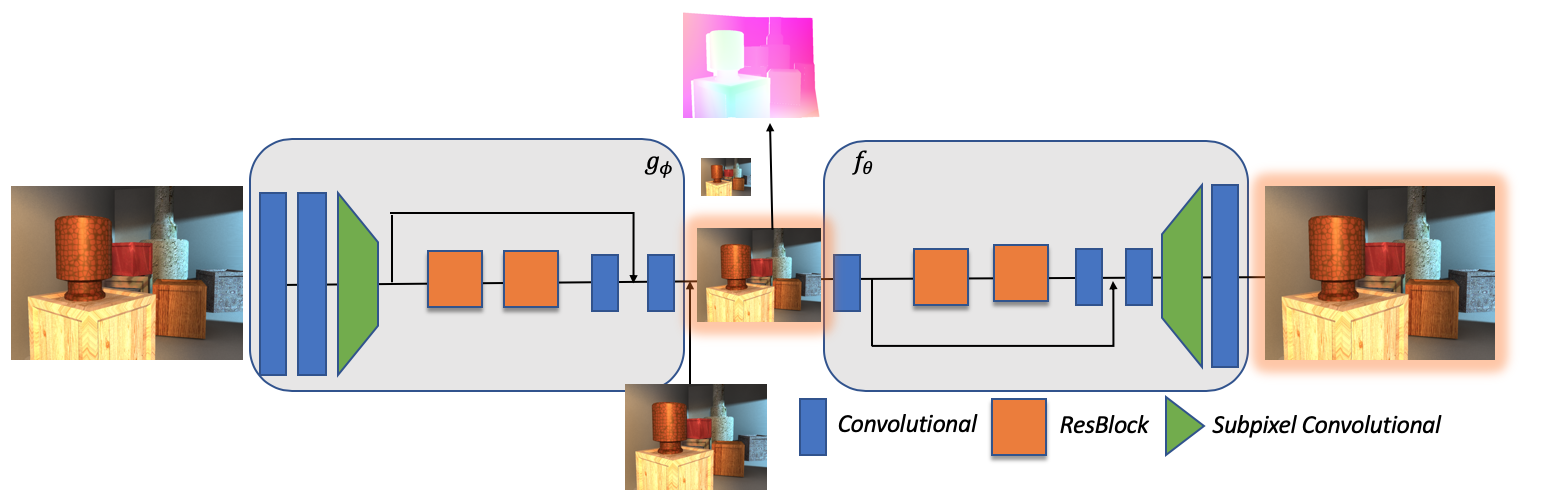
\includegraphics[width=14cm]{figures/architecture_video_flow}
	\caption{Design for \ac{TAD} video super-resolution architecture for optical flow reconstruction. }
  \label{fig:architecture_video_flow}
\end{figure}

\begin{figure}[!ht]
	\centering
	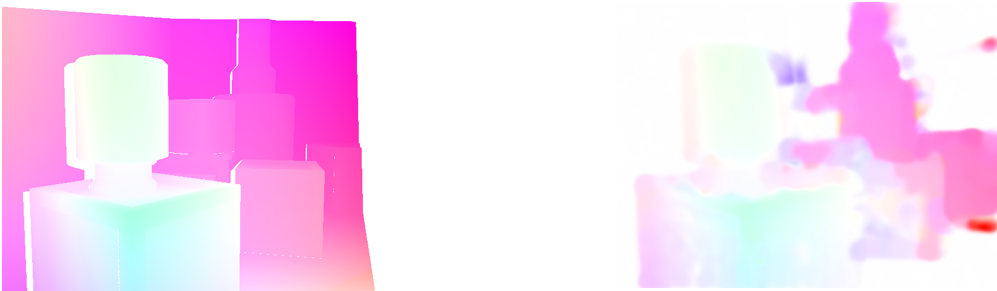
\includegraphics[width=10cm]{figures/flow}
	\caption{Optical flow reconstruction: Groundtruth (left) and reconstructed
  image (right).}
  \label{fig:flow}
\end{figure}

\section*{SOFVSR model selection and working principle}
Wang et al. \cite{LFVSRTHROFE} (SOFVSR) implemented an end-to-end trainable approach to predict both, the \ac{HR} frame as well as the HR optical flow. Therefore, first the HR optical flow is inferred in a coarse-to-fine manner, then motion compensation is performed according to the HR optical flows and finally, the compensated LR inputs are fed to a super-resolution network to generate the HR frame estimate (comp. \myfigref{fig:sofvsr}).

\begin{figure}[!ht]
	\centering
	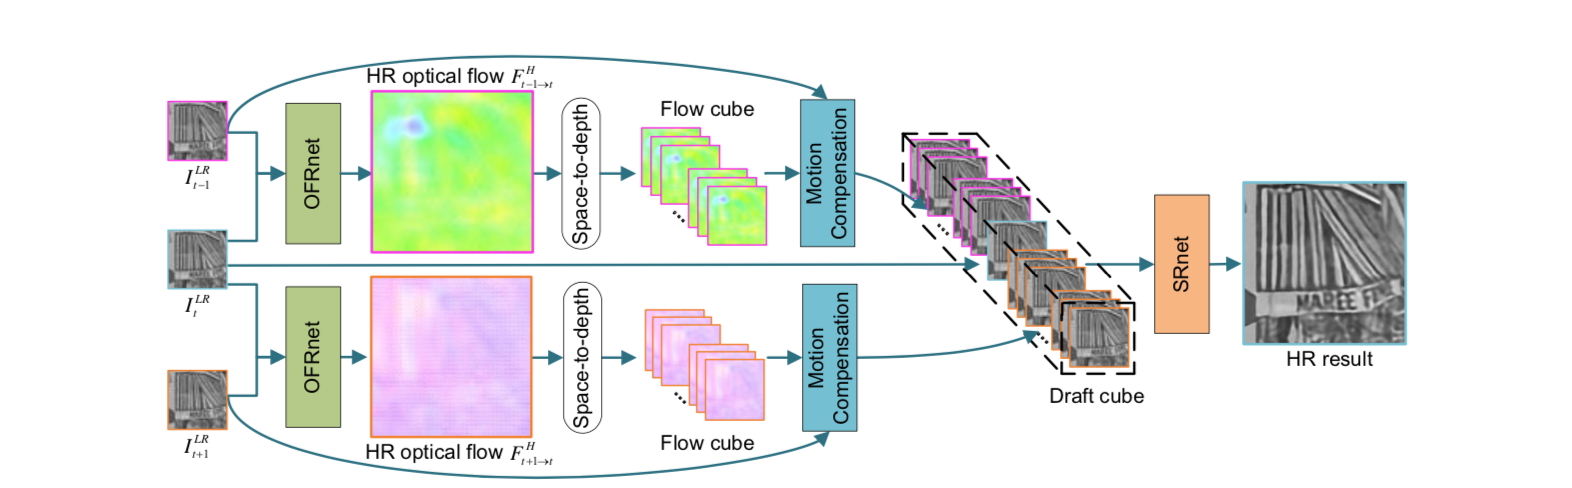
\includegraphics[width=14cm]{figures/sofvsr}
	\caption{Overview of SOFVSR pipeline \cite{LFVSRTHROFE}.}
  \label{fig:sofvsr}
\end{figure}

The SOFVSR model was selected based on a combination of criteria such as the stated reconstruction performance (PSNR) and runtime, the closeness to
state-of-the-art and the availability of a PyTorch open-source implementation.

\begin{figure}[!ht]
	\centering
	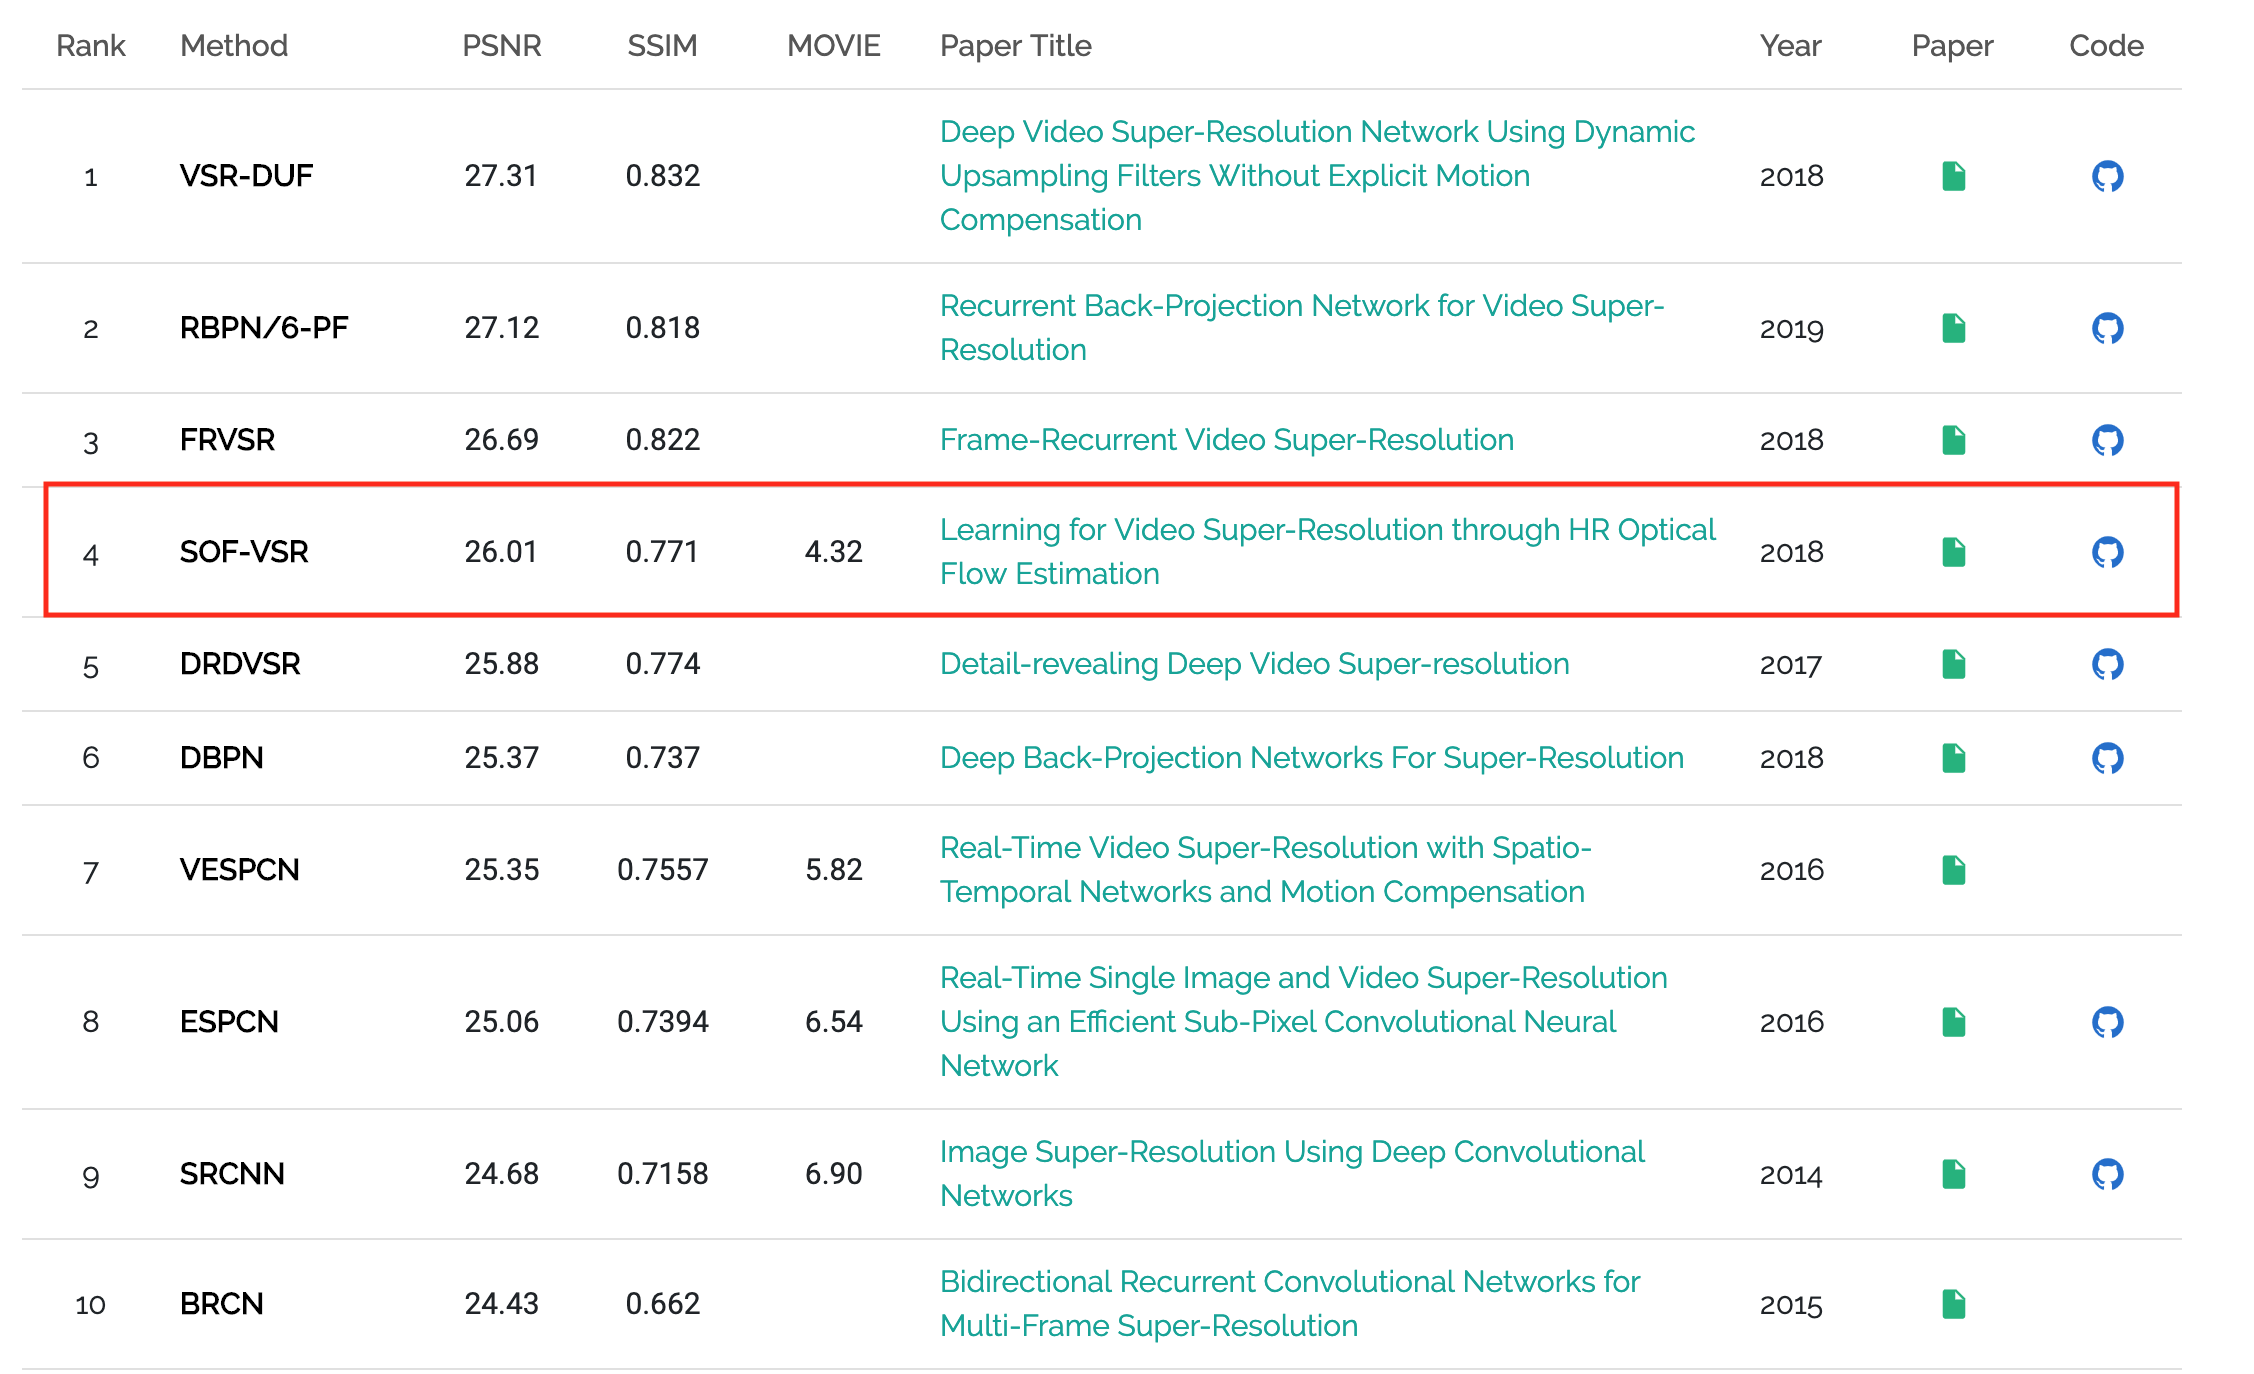
\includegraphics[width=14cm]{figures/sofvsr_selection}
	\caption{Comparison of several \ac{VSR} methods according to PapersWithCode.}
  \label{fig:sofvsr_selection}
\end{figure}

\section*{List of Architectures}
For the sake of simplicity in the following only the models used for the \ac{SISR} task are displayed. The models used for the other tasks are basically similar, apart from the task specific model constraints, e.g. the lack of subpixel convolutions in \ac{IC} models as the image dimensions are kept, just its number of channels is downscaled. However, the following list contains the most important models, that were used for evaluation.   

\begin{figure}[!ht]
\centering
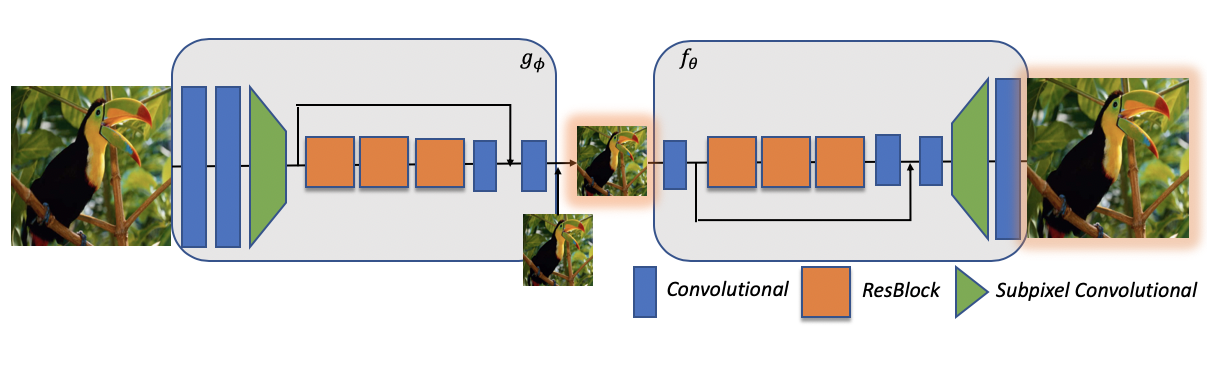
\includegraphics[width=14cm]{figures/architecture_baseline.png}
\caption{Model architecture - $aetad\_baseline$ (Kim et al. \cite{TAID})}
\end{figure}

\begin{figure}[!ht]
\centering
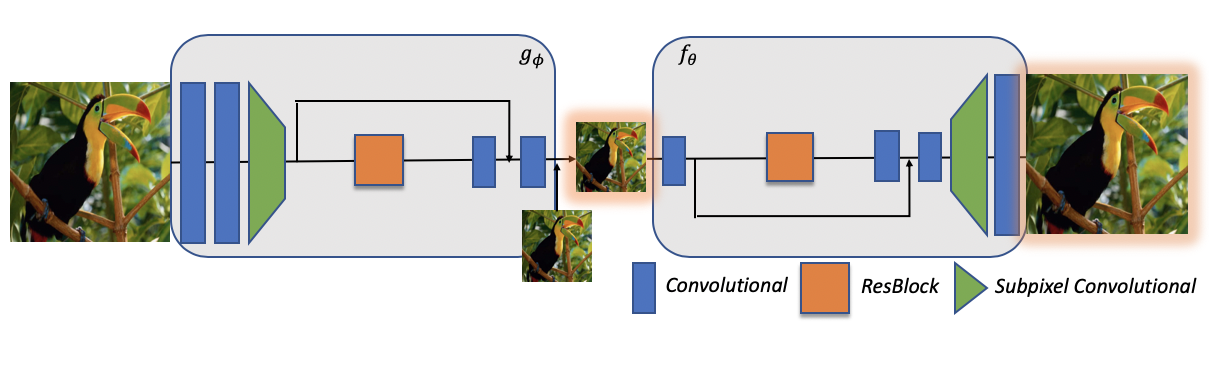
\includegraphics[width=14cm]{figures/architecture_very_small.png}
\caption{Model architecture - $aetad\_very\_small$}
\end{figure}

\begin{figure}[!ht]
\centering
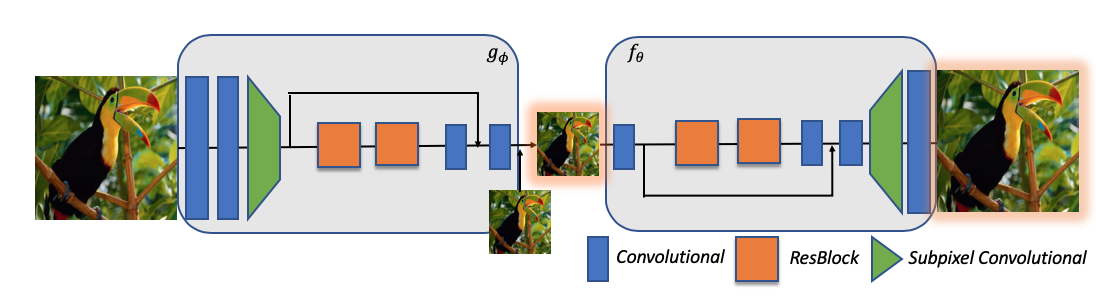
\includegraphics[width=14cm]{figures/architecture_small.png}
\caption{Model architecture - $aetad\_small$}
\end{figure}

\begin{figure}[!ht]
\centering
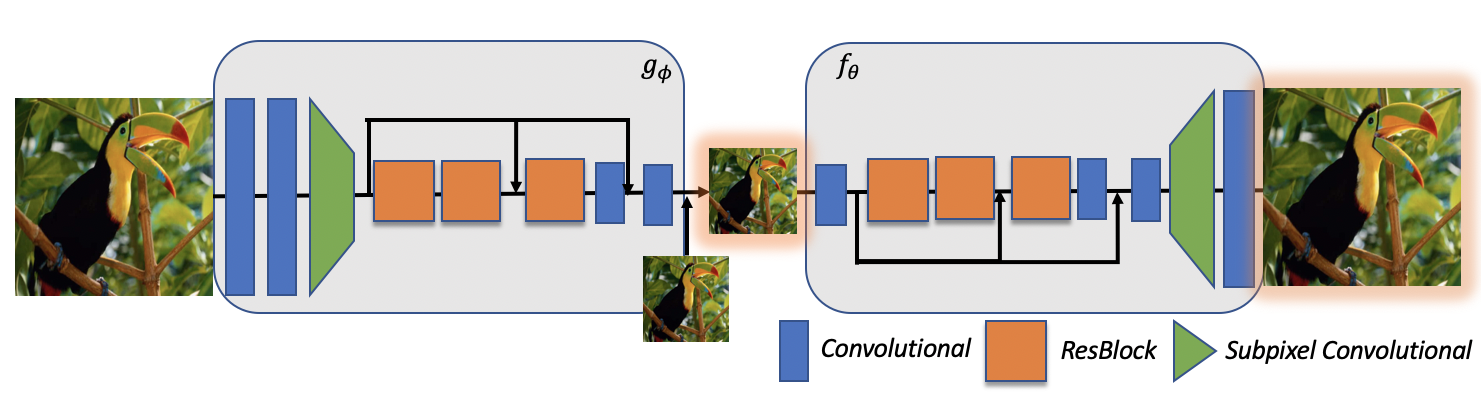
\includegraphics[width=14cm]{figures/architecture_skip2.png}
\caption{Model architecture - $aetad\_skip2$}
\end{figure}

\begin{figure}[!ht]
\centering
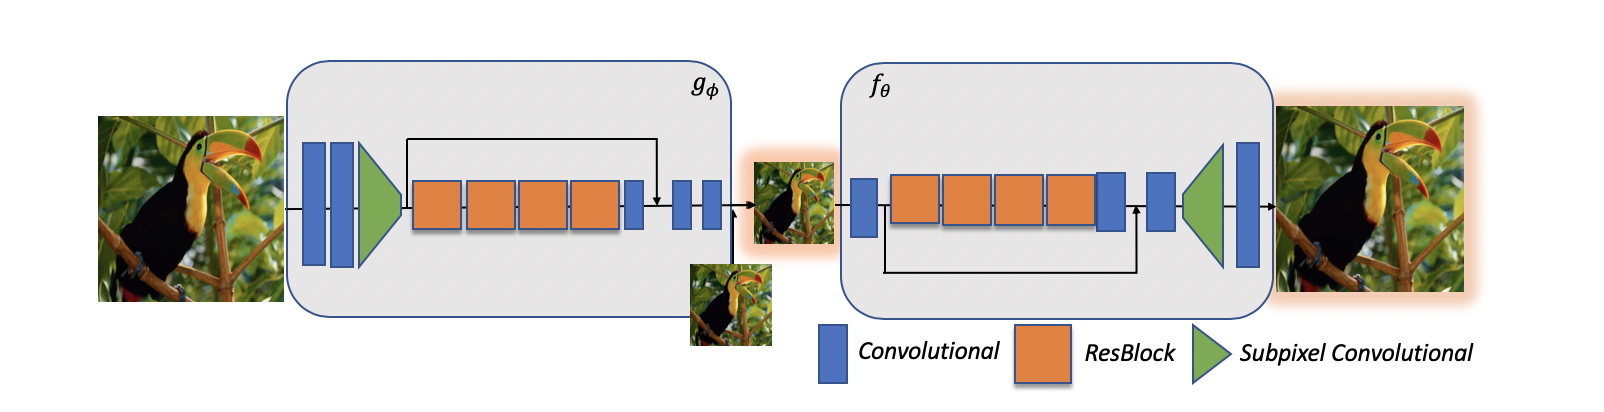
\includegraphics[width=14cm]{figures/architecture_large.png}
\caption{Model architecture - $aetad\_large$}
\end{figure}

\begin{figure}[!ht]
\centering
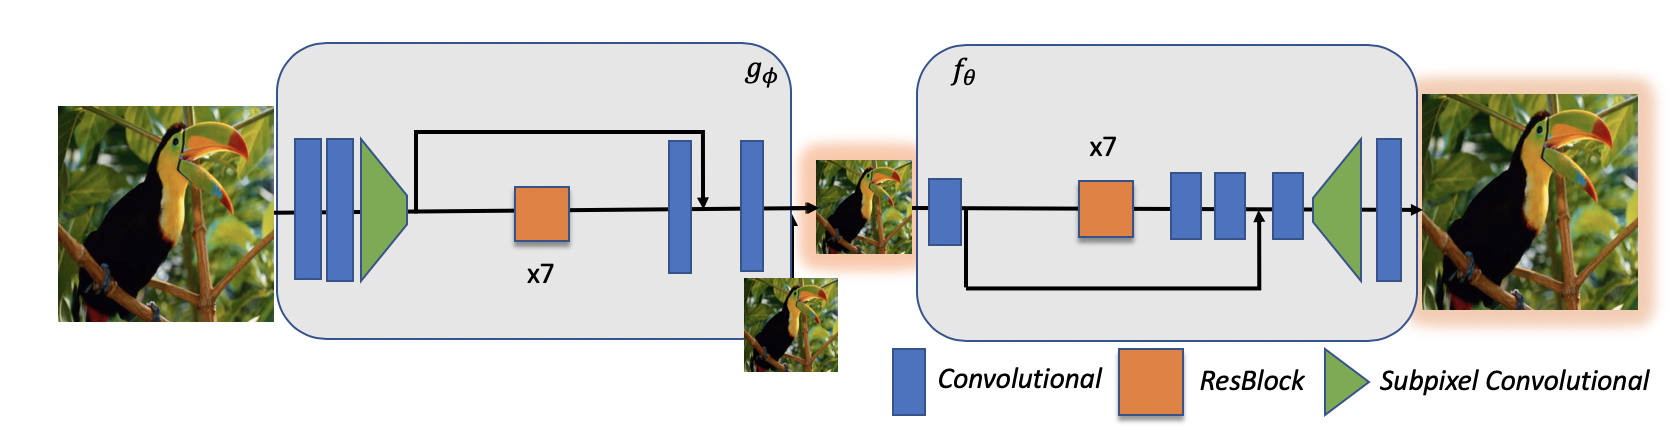
\includegraphics[width=14cm]{figures/architecture_very_large2.png}
\caption{Model architecture - $aetad\_very\_large2$}
\end{figure}


\begin{figure}[!ht]
\centering
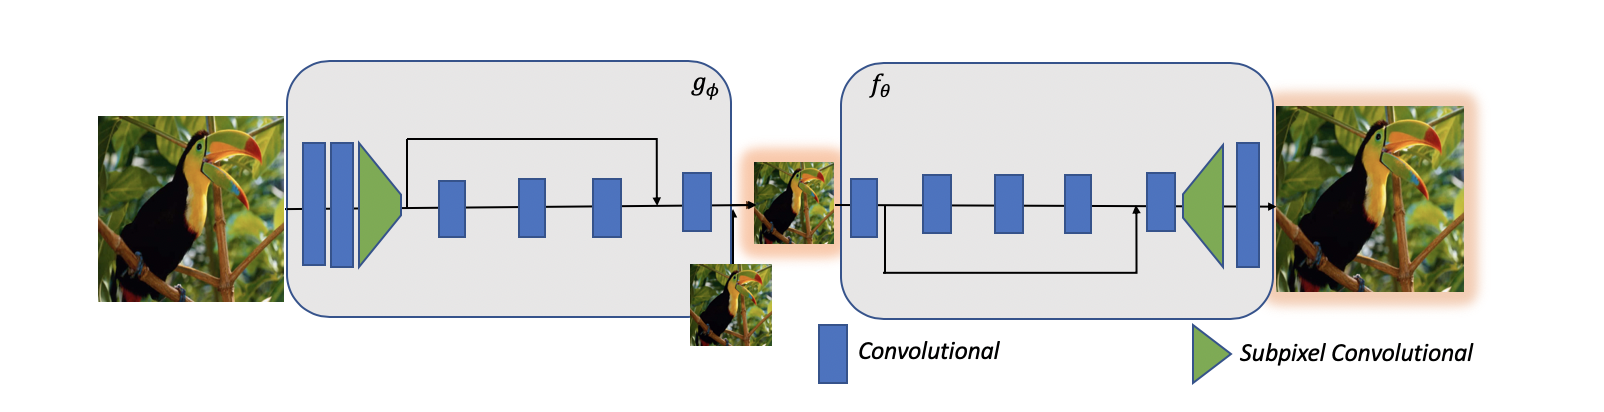
\includegraphics[width=14cm]{figures/architecture_conv_only.png}
\caption{Model architecture - $aetad\_conv\_only$}
\end{figure}

\begin{figure}[!ht]
\centering
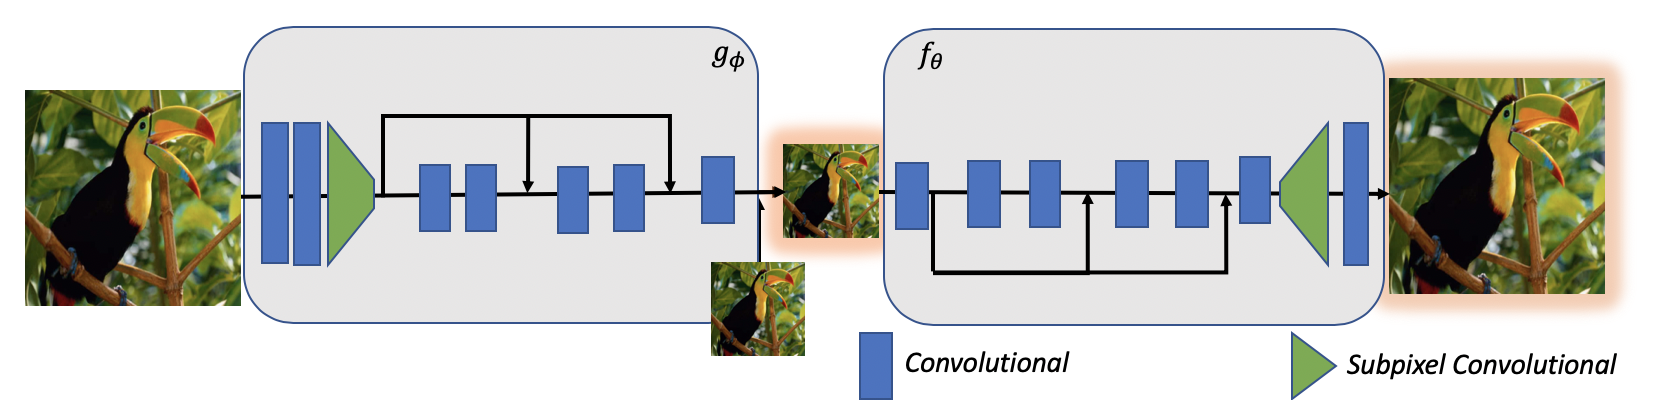
\includegraphics[width=14cm]{figures/architecture_conv_only_large.png}
\caption{Model architecture - $aetad\_conv\_only\_large$}
\end{figure}

\begin{figure}[!ht]
\centering
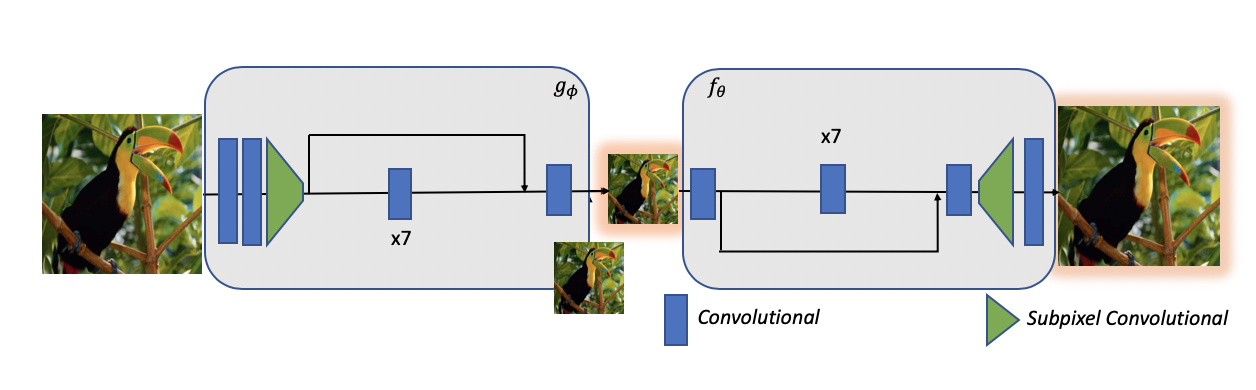
\includegraphics[width=14cm]{figures/architecture_conv_only_very_large.png}
\caption{Model architecture - $aetad\_conv\_only\_very\_large$}
\end{figure}

\clearpage
\section*{List of Experiments}

\begin{table}[!ht]
\centering
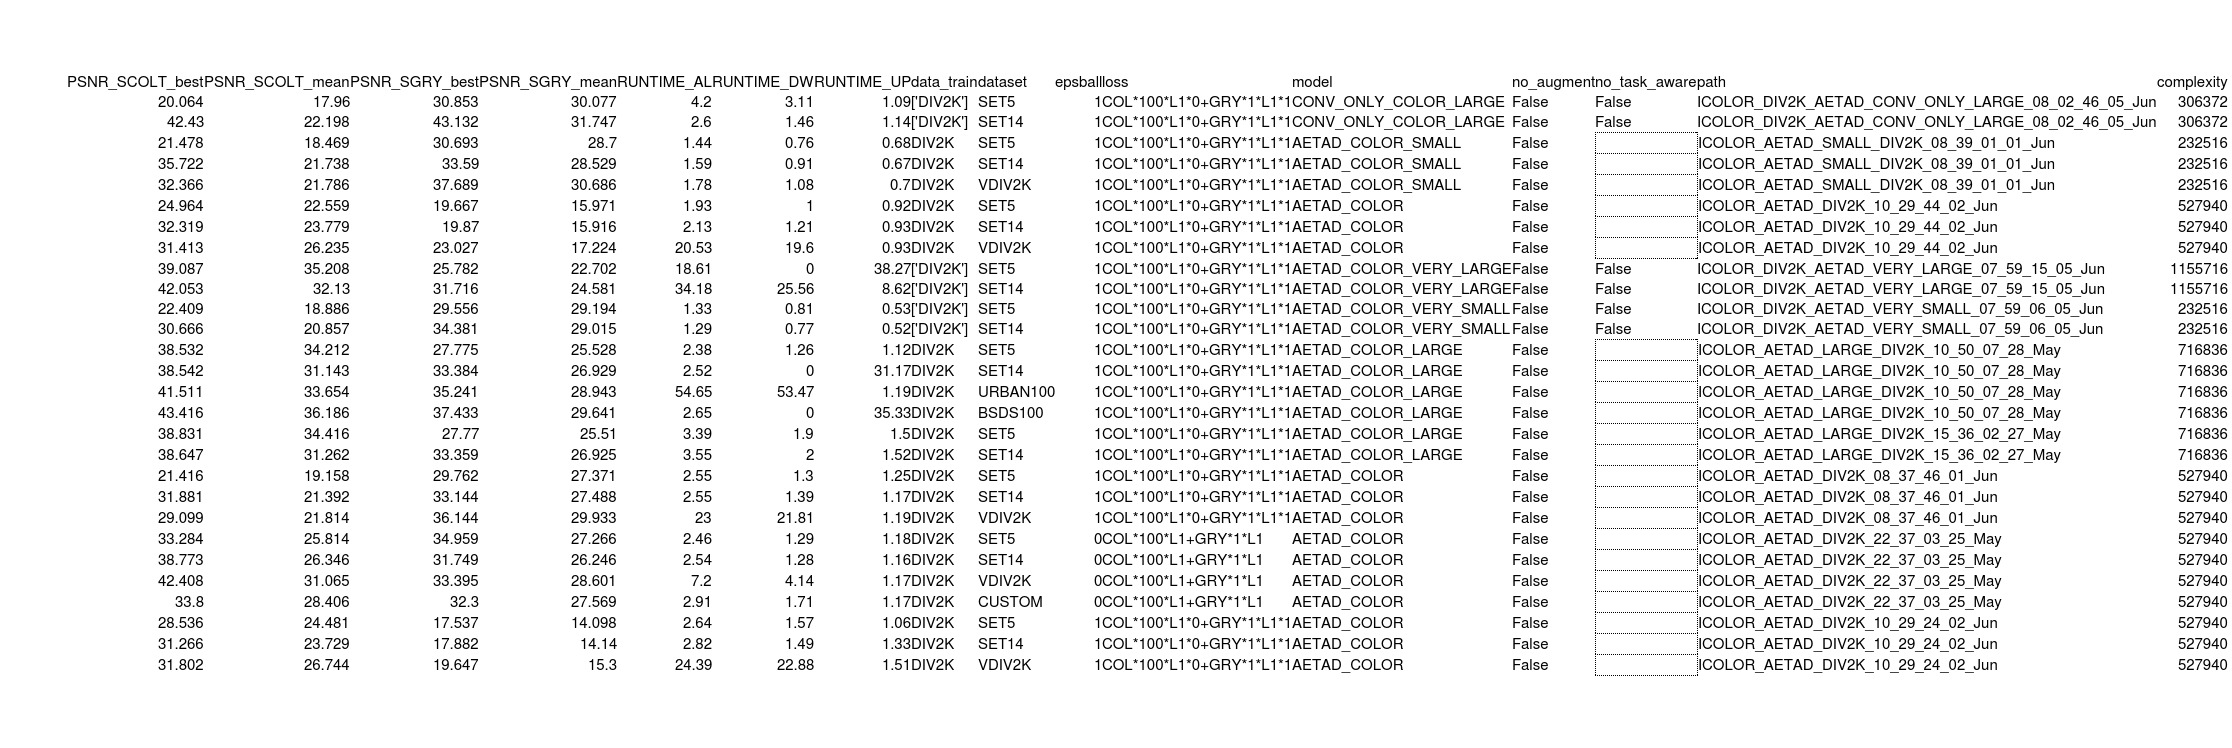
\includegraphics[width=16cm]{figures/data_ic}
\caption{List of important (non-complete) \ac{IC} experiments.}
\label{table:experiments_ic}
\end{table}

\begin{table}[!ht]
\centering
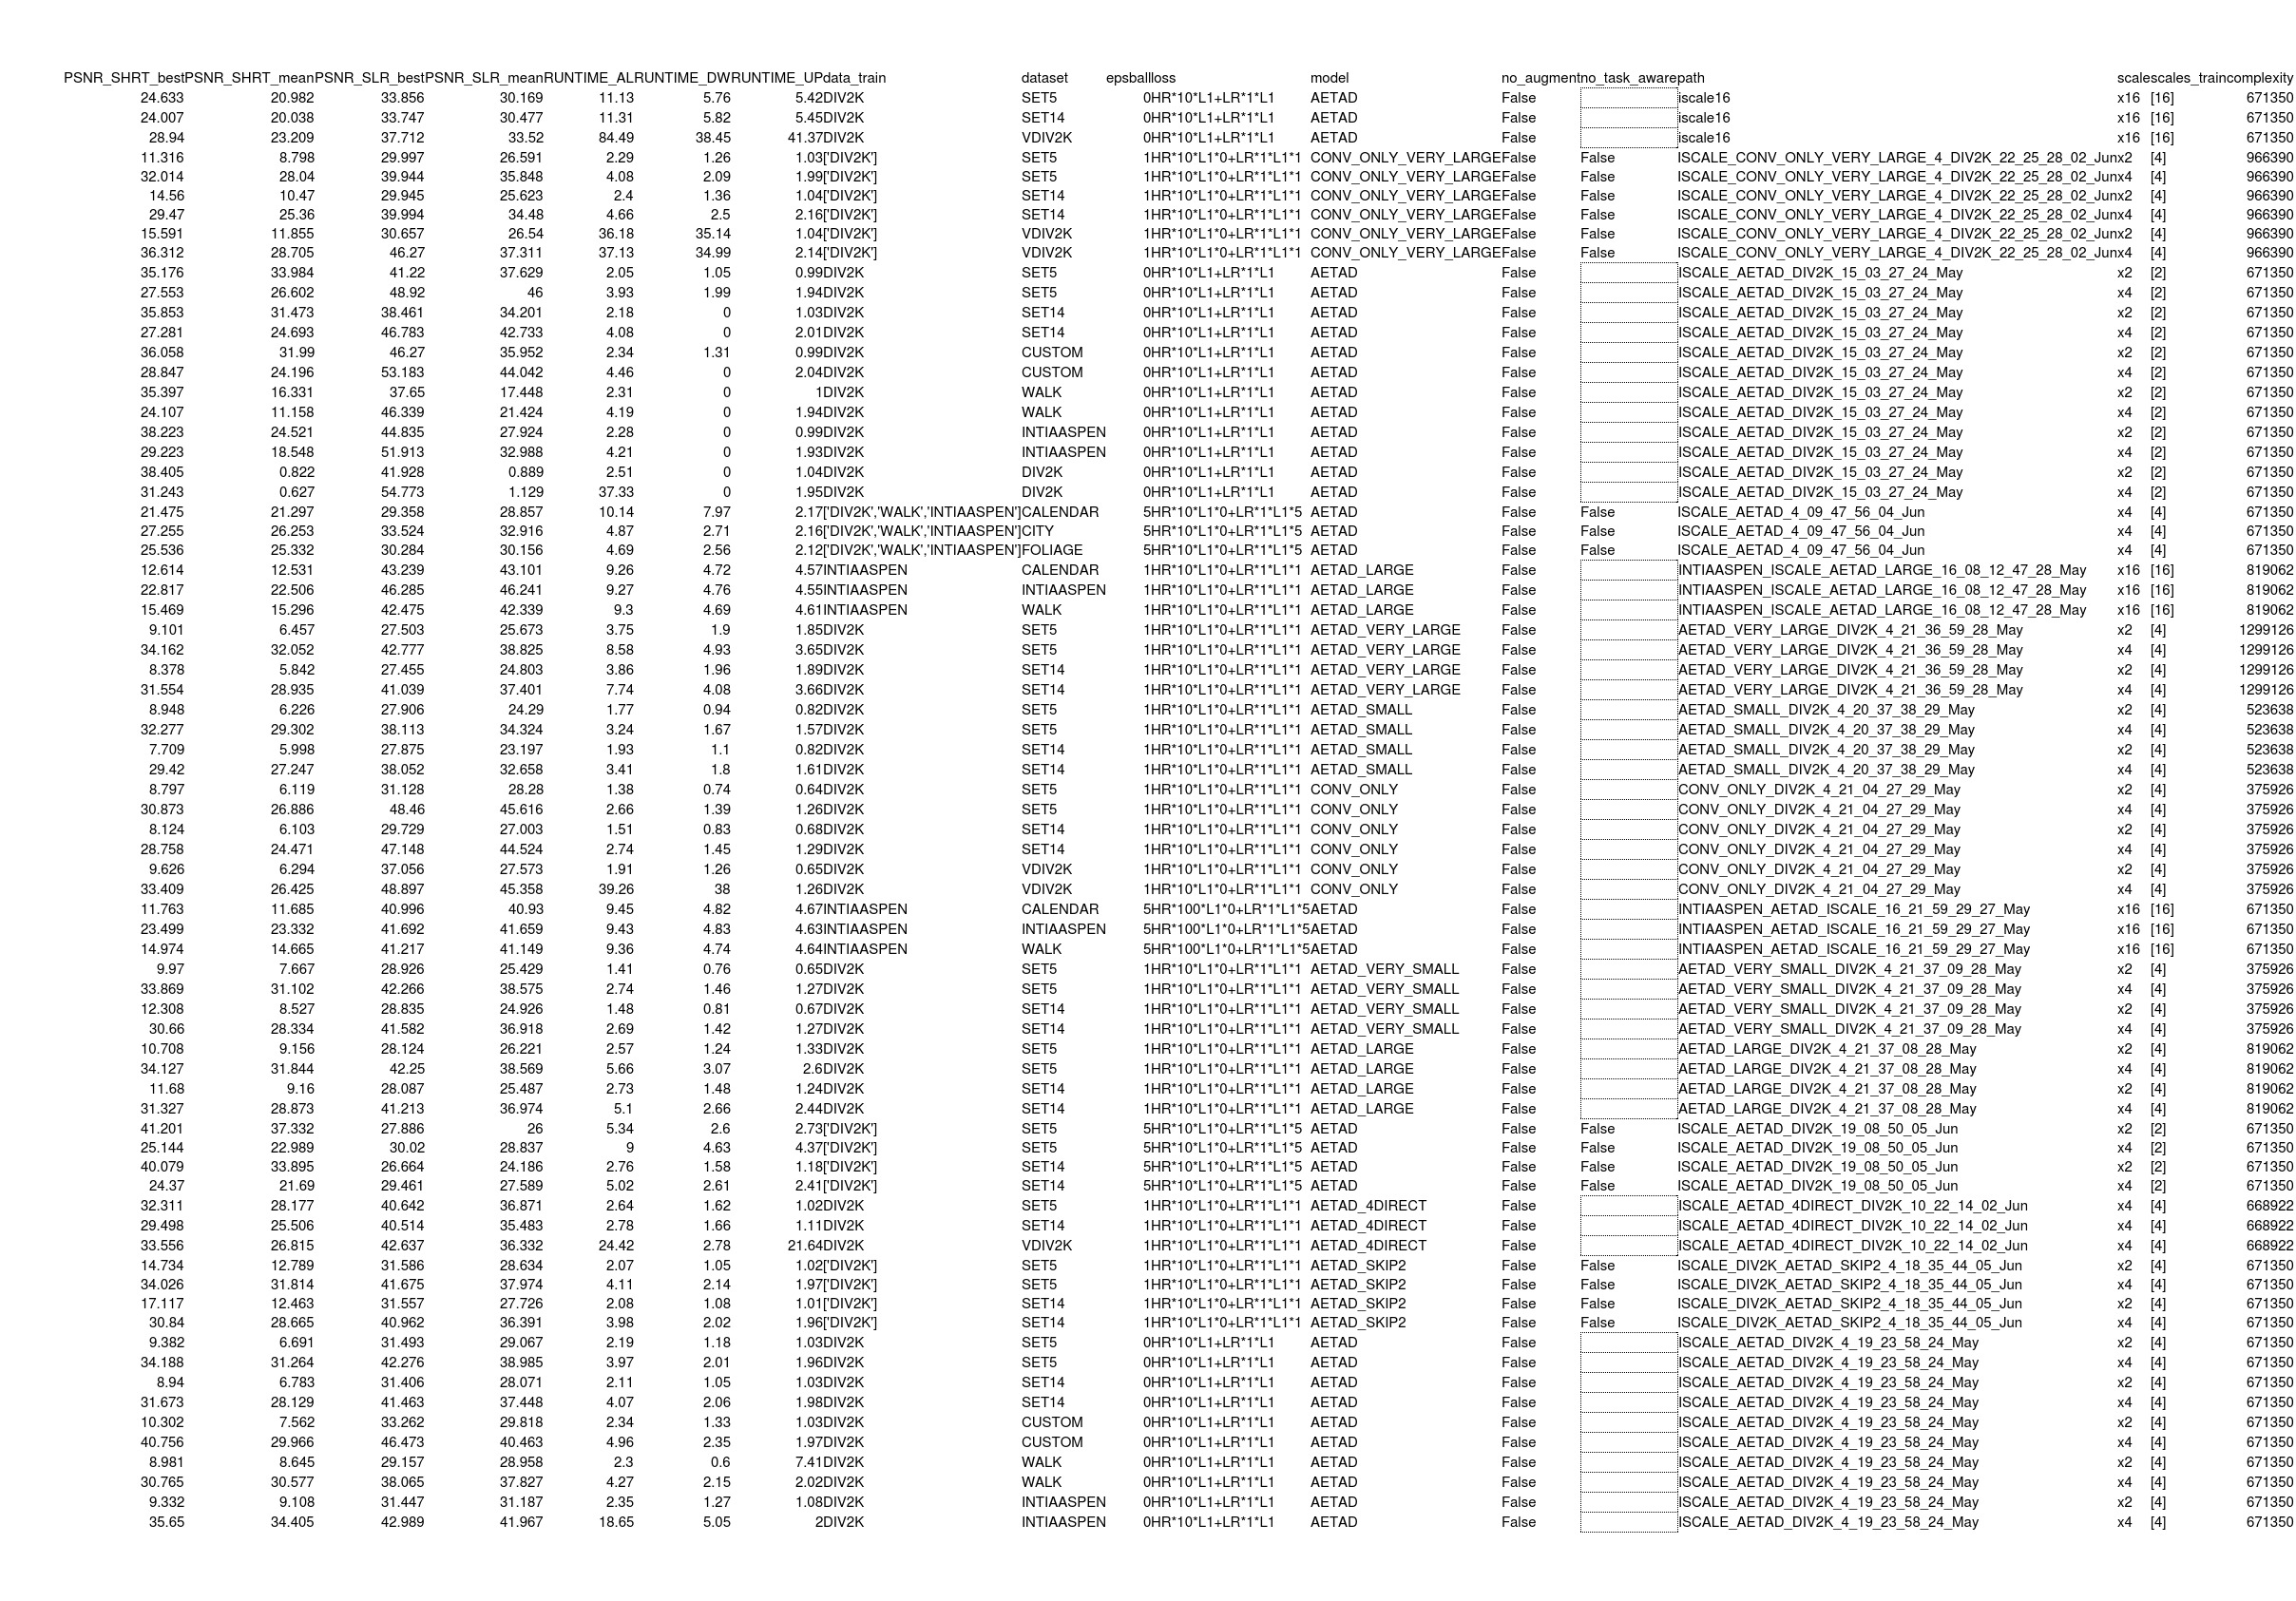
\includegraphics[width=16cm]{figures/data_sisr}
\caption{List of important (non-complete) \ac{SISR} experiments.}
\label{table:experiments_sisr}
\end{table}

\begin{table}[!ht]
\centering
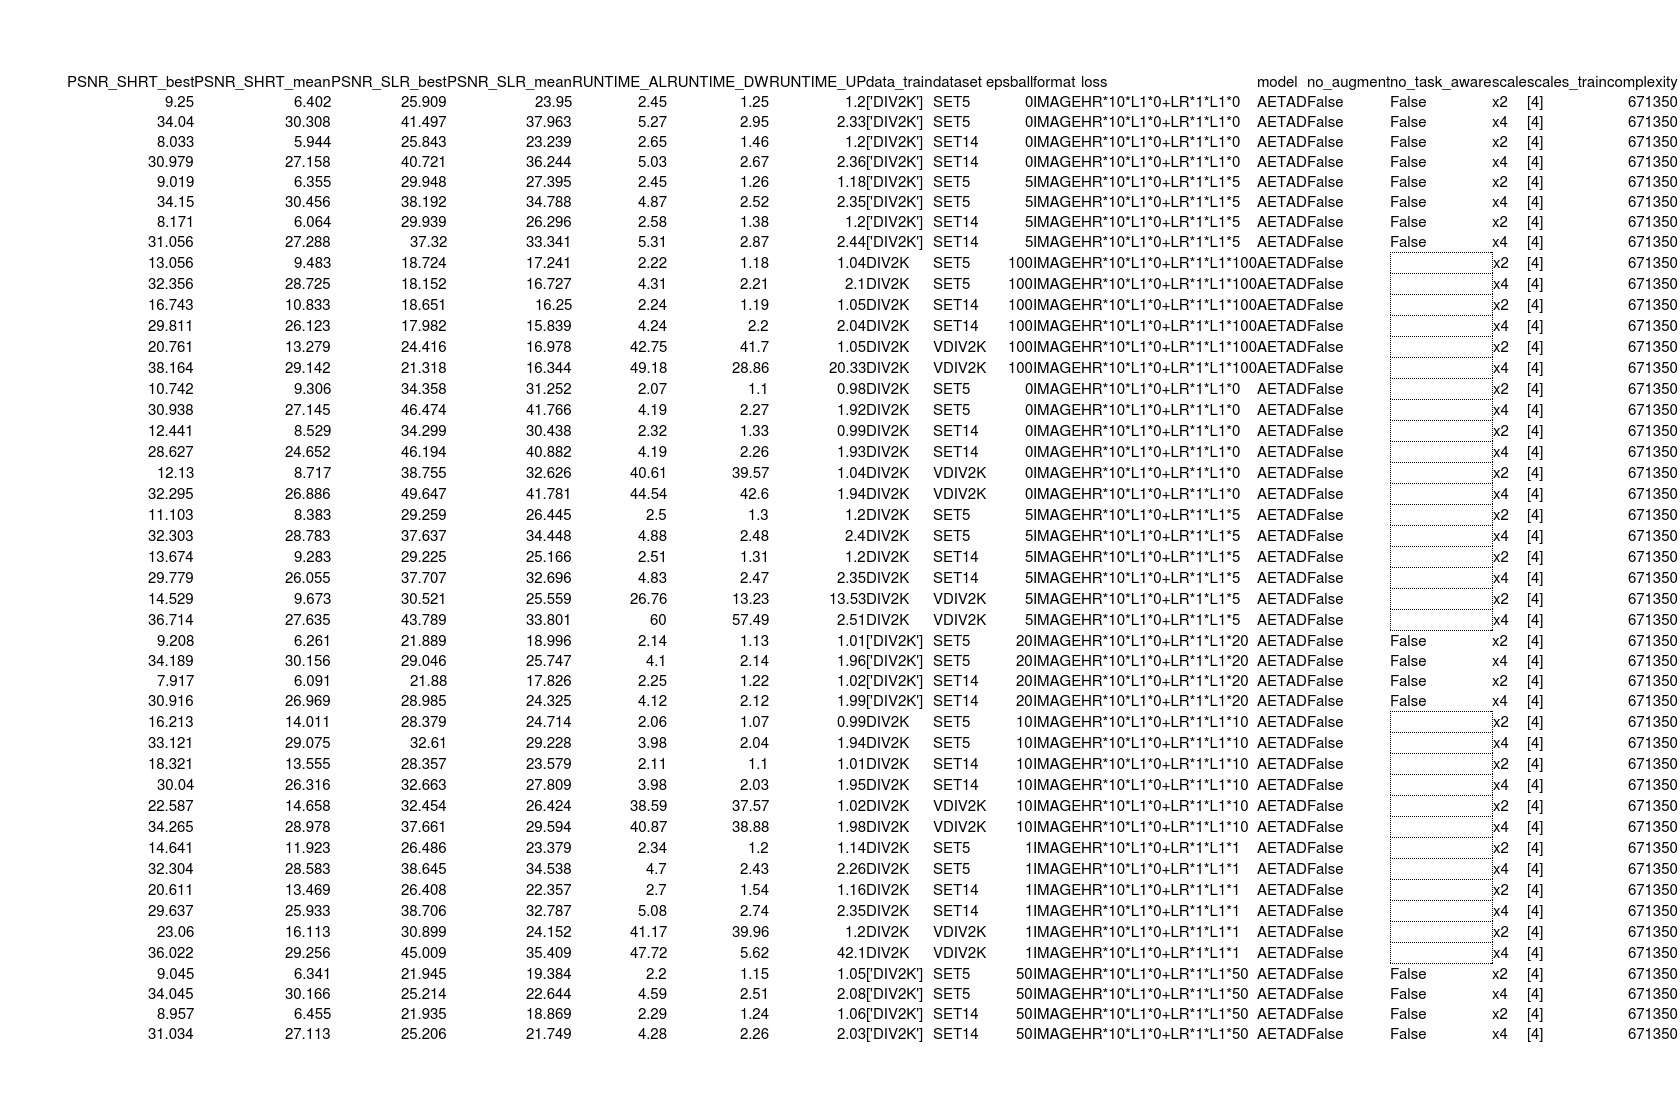
\includegraphics[width=16cm]{figures/data_epsilon_ball.jpg}
\caption{List of important (non-complete) perturbation experiments.}
\label{table:experiments_epsilon}
\end{table}